\documentclass[border={0.1cm -0.1cm 0.1cm 0.1cm}]{standalone}  %E,S,W,N

\usepackage{amssymb}
\usepackage{amsmath}
\usepackage{tikz}
\usetikzlibrary{shapes} %for node shapes
\usetikzlibrary{decorations.text} %for curvy text

%Central argument in Anti-Oedipus, by Dennis Schulting
%https://twitter.com/AmcCritique/status/1410167574801887240

\begin{document}
	
	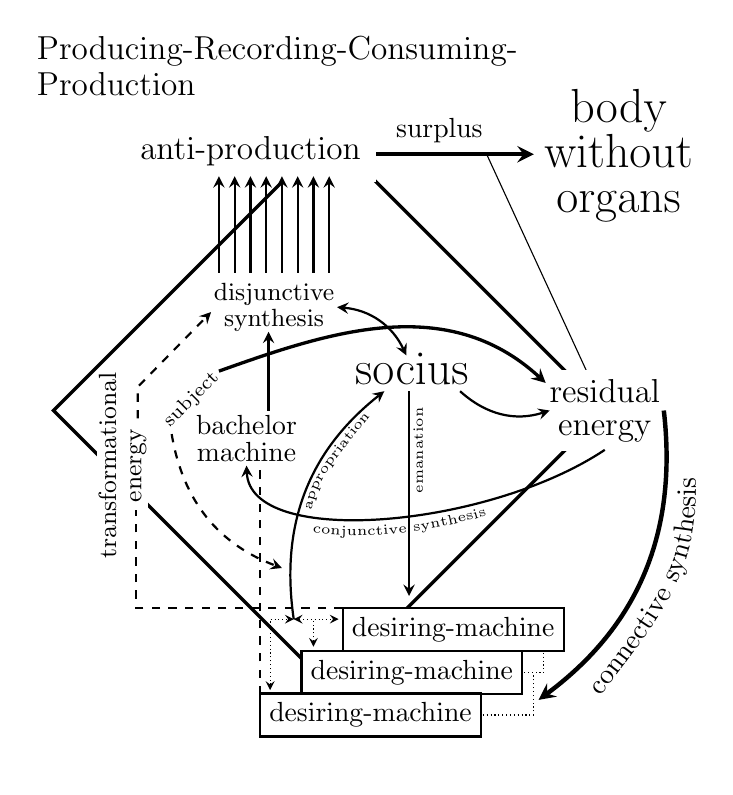
\begin{tikzpicture}[very thick]
	\def\n{3.5}
	\draw (0,\n)--(\n,0)--(0,-\n)--(-\n,0)--cycle;	%main square
	
	%TOP
	%\node[align=right] at (-1.1*\n,1.25*\n) {\large Producing- \\\large Recording- \\\large Consuming- \\[0.25mm]\large Production};
	\node[align=left,right] at (-1.1*\n,1.25*\n) {\large Producing-Recording-Consuming- \\[0.25mm]\large Production};
	%
	\draw[ultra thick,->,>=stealth] (0,0.93*\n)--(1.4,0.93*\n) node[above] {surplus}--(2.6,0.93*\n);
	\draw[thin] (2,0.93*\n)--(\n,0);
	\node[rectangle,fill=white,inner sep=5.6] at (-1,0.94*\n) {\large anti-production};
	%
	\foreach \i in {0,...,7} \draw [->,>=stealth,thick] (-0.2*\i,0.5*\n)--(-0.2*\i,0.85*\n);
	\node[align=center] at (-0.2*3.5,0.375*\n) {\small disjunctive \\[-1mm]\small synthesis};
	
	%RIGHT
	\node[align=center,fill=white] at (\n,0) {\large residual \\\large energy};
	\node[align=center] at (1.05*\n,0.925*\n) {\LARGE body \\\LARGE without \\[1.5mm]\LARGE organs};
	\draw[->,>=stealth,ultra thick] (4.25,0) to[bend left] (0.76*\n,-1.05*\n);
	\draw [decorate, decoration={text along path, text align=center, text={|\normalsize|connective synthesis}}] (2.75,-4.5) .. controls (4.75,-2) .. (4.6,0.25);
	%
	\draw[->,>=stealth,thick] (\n,-0.5) .. controls (2,-1.5) and (-1,-1.75) .. (-0.3*\n,-0.2*\n);
	\draw [decorate, decoration={text along path, text align=center, text={|\tiny|conjunctive synthesis}}] (-0.3*\n-0.2,-0.2*\n) .. controls (-1.25,-2) and (1.75,-1.75) .. (\n-0.15,-0.75);
	
	%LEFT
	\node[rotate=90,align=center,fill=white,inner sep=0.75] at (-0.75*\n,-0.2*\n) {\small transformational \\[-1mm]\small energy};
	\draw[->,>=stealth,dashed,thick] (-2.43,-0.1)--(-2.43,0.3)--(-1.5,1.25);
	
	%BOTTOM
	%long dashed lines
	\draw[dashed,thick] (0.45*\n-0.1375,-0.717*\n)--(-0.7*\n,-0.717*\n)--(-0.7*\n,-0.36*\n);
	\draw[dashed,thick] (-0.25*\n,-1.105*\n+0.05)--(-0.25*\n,-0.21*\n);
	%
	%dotted lines connecting blocks
	\draw[densely dotted,thin] (0.45*\n+1.15,-0.795*\n)--++(0,-0.55)--++(-1,0);
	\draw[densely dotted,thin] (0.15*\n,-1.105*\n)--++(2.07,0)--++(0,0.52);
	%
	\node[rectangle,fill=white,draw=black,thick] at (0.45*\n,-0.795*\n) {desiring-machine};
	\node[rectangle,fill=white,draw=black,thick] at (0.30*\n,-0.950*\n) {desiring-machine};
	\node[rectangle,fill=white,draw=black,thick] at (0.15*\n,-1.105*\n) {desiring-machine};
	%
	\draw[<->,>=stealth,densely dotted,thin] (-0.2,-3)--(-0.2,-2.65)--(0.12,-2.65);
	\draw[<->,>=stealth,densely dotted,thin] (-0.75,-3.55)--(-0.75,-2.65)--(-0.45,-2.65);
	\draw[->,>=stealth,densely dotted,thin] (-0.22,-2.65)--(-0.45,-2.65);
	%
	\draw[->,>=stealth,thick] (-0.45,-2.65) to[bend left] (0.2*\n,0.07*\n);
	%\draw [decorate, decoration={text along path, text align=center, text={|\tiny|appropriation}}] (-0.25,-1.75) .. controls (-0.25,-1) .. (0.5,0);
	\draw [decorate, decoration={text along path, text align=center, text={|\tiny|appropriation}}] (-0.25,-1.4) .. controls (-0.15,-0.9) .. (0.6,0.03);
	
	%MIDDLE
	\node[align=center] at (-0.3*\n,-0.1*\n) {bachelor \\[-0.75mm] machine};
	\draw[->,>=stealth,thick] (-0.22*\n,0*\n)--++(0,1);
	%
	\node at (-0.5*\n,0.04*\n) {\rotatebox{45}{\scriptsize subject}};
	\draw[->,>=stealth,very thick] (-1.4,0.5) .. controls (0,1) and (1.5,1.5) .. (2.75,0.35);
	\draw[->,>=stealth,thick,dashed] (-2,-0.3) to[bend right] (-0.6,-2);
	%
	\node at (0.3*\n,0.15*\n) {\LARGE socius};
	\draw[<->,>=stealth,thick] (0.28*\n,0.2*\n) to[bend right] (0.1,0.375*\n);
	\draw[->,>=stealth,thick] (0.475*\n,0.07*\n) to[bend right] (0.8*\n,0);
	\draw[->,>=stealth,thick] (0.29*\n,0.07*\n)--++(0,-0.75) node[right,xshift=-0.75mm] {\rotatebox{90}{\tiny emanation}} --++(0,-1.85);
	
	%\draw[help lines] (-5,-5) grid (5,5);
	\end{tikzpicture}
	
\end{document}